
\documentclass[paper=a4, fontsize=11pt]{scrartcl} % A4 paper and 11pt font size

\usepackage{times, epsfig, graphicx, amsmath, amssymb, floatrow, booktabs, url, multirow,comment}
\usepackage[margin=0.5in]{geometry}
\graphicspath{ {images/} }
\usepackage[T1]{fontenc} % Use 8-bit encoding that has 256 glyphs
\usepackage{fourier} % Use the Adobe Utopia font for the document - comment this line to return to the LaTeX default
\usepackage[english]{babel} % English language/hyphenation
\usepackage[hidelinks]{hyperref}
\usepackage{sectsty} % Allows customizing section commands
%\allsectionsfont{\centering \normalfont\scshape} % Make all sections centered, the default font and small caps

\usepackage{fancyhdr} % Custom headers and footers
\pagestyle{fancyplain} % Makes all pages in the document conform to the custom headers and footers
\fancyhead{} % No page header - if you want one, create it in the same way as the footers below
\fancyfoot[L]{} % Empty left footer
\fancyfoot[C]{} % Empty center footer
\fancyfoot[R]{\thepage} % Page numbering for right footer
\renewcommand{\headrulewidth}{0pt} % Remove header underlines
\renewcommand{\footrulewidth}{0pt} % Remove footer underlines
\setlength{\headheight}{13.6pt} % Customize the height of the header


\numberwithin{equation}{section} % Number equations within sections (i.e. 1.1, 1.2, 2.1, 2.2 instead of 1, 2, 3, 4)
\numberwithin{figure}{section} % Number figures within sections (i.e. 1.1, 1.2, 2.1, 2.2 instead of 1, 2, 3, 4)
\numberwithin{table}{section} % Number tables within sections (i.e. 1.1, 1.2, 2.1, 2.2 instead of 1, 2, 3, 4)

\setlength{\parindent}{0pt} % Removes all indentation from paragraphs - comment this line for an assignment with lots of text

%----------------------------------------------------------------------------------------
%   TITLE SECTION
%----------------------------------------------------------------------------------------

\newcommand{\horrule}[1]{\rule{\linewidth}{#1}} % Create horizontal rule command with 1 argument of height

\title{
\normalfont \normalsize
\textsc{CVC@CentraleSupelec and Schneider Electric} \\ [25pt] % Your university, school and/or department name(s)
\horrule{0.5pt} \\[0.4cm] % Thin top horizontal rule
\huge Motor Control Dataset Statistics \\ % The assignment title
\horrule{2pt} \\[0.5cm] % Thick bottom horizontal rule
}

\author{Sagar Verma} % Your name

\date{\normalsize\today} % Today's date or a custom date

\begin{document}

\maketitle % Print the title

%----------------------------------------------------------------------------------------
%   PROBLEM 1
%----------------------------------------------------------------------------------------

\section{Data Statistics}

  \begin{figure}[H]
     \centering
      \href{https://plot.ly/~versag/20/#/}{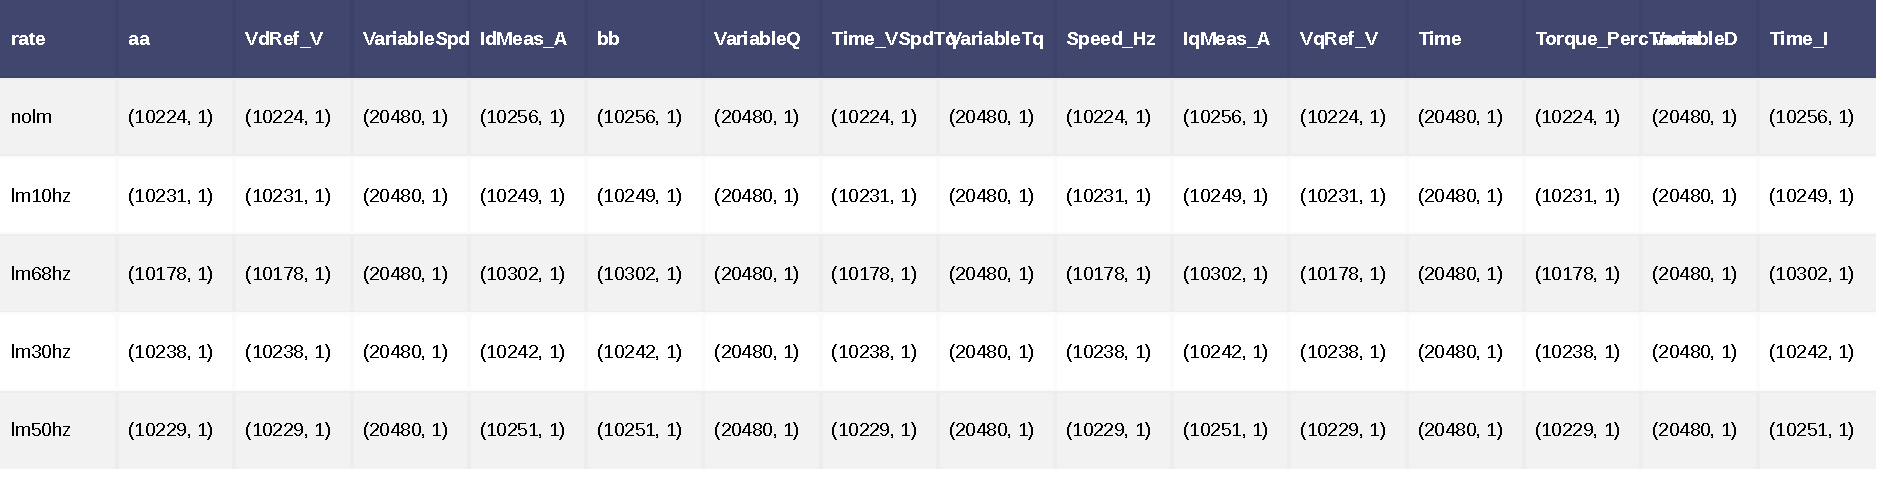
\includegraphics[width=1\linewidth]{dimension_of_features_in_dataset}}
        \caption{Dimensions of Features in the Dataset}
  \end{figure}

  \begin{figure}[H]
    \centering
      \href{https://plot.ly/~versag/24/#/}{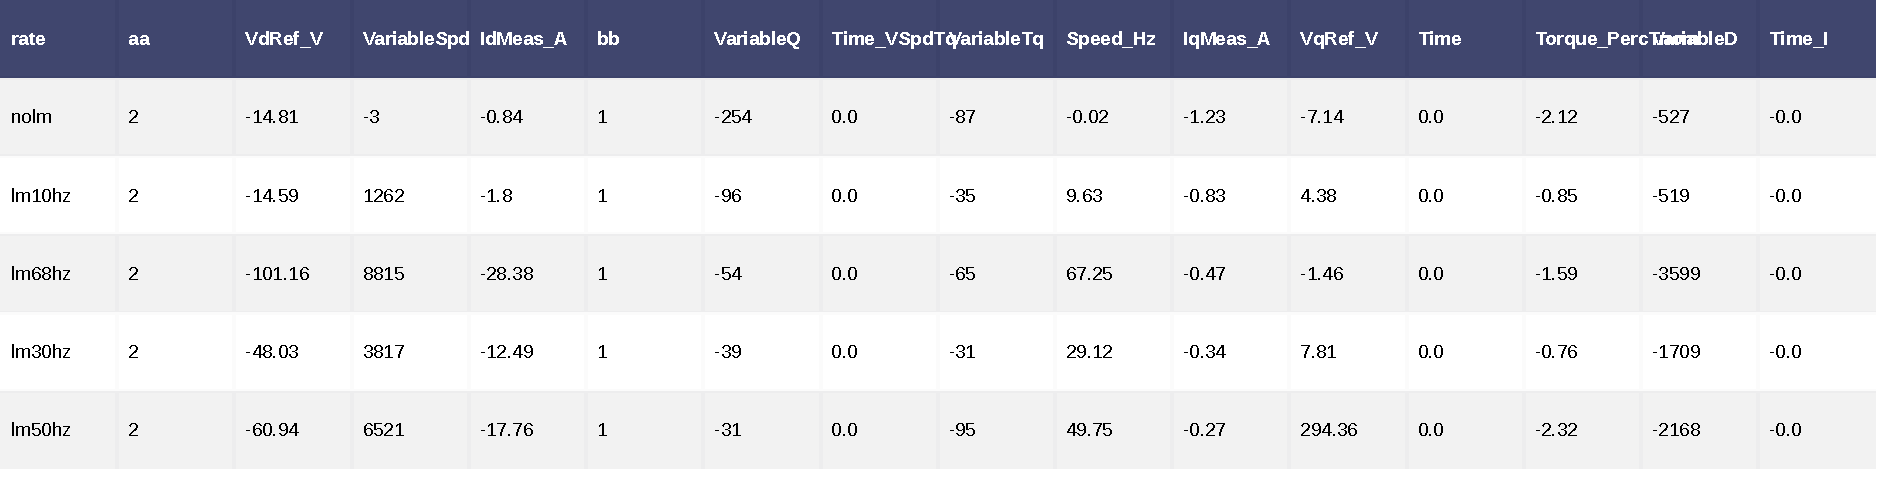
\includegraphics[width=1\linewidth]{min_values_of_features_in_dataset}}
        \caption{Min Value of Features in the Dataset}
  \end{figure}

  \begin{figure}[H]
    \centering
      \href{https://plot.ly/~versag/22/#/}{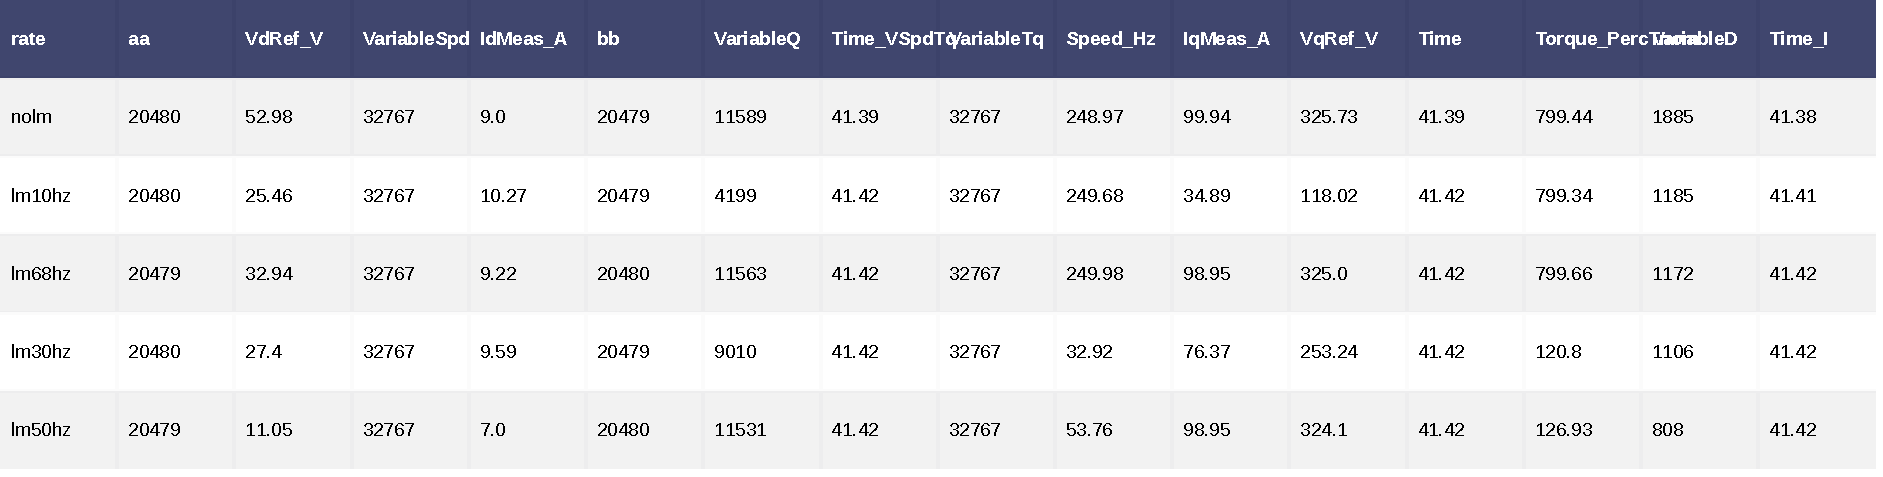
\includegraphics[width=1\linewidth]{max_values_of_features_in_dataset}}
        \caption{Max Value of Features in the Dataset}
  \end{figure}

  \begin{figure}[H]
    \centering
    \href{https://plot.ly/~versag/46/#/}{  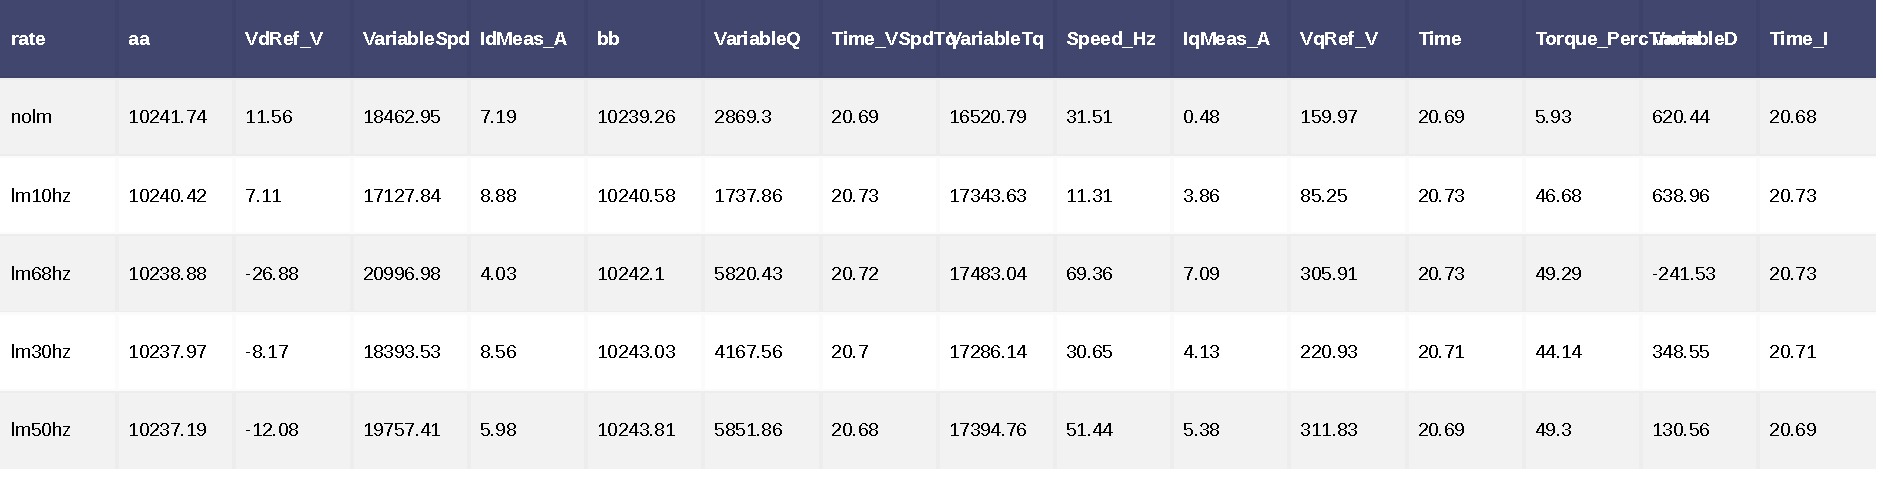
\includegraphics[width=1\linewidth]{mean_values_of_features_in_dataset}}
        \caption{Mean Value of Features in the Dataset}
  \end{figure}

  \begin{figure}[H]
    \centering
      \href{https://plot.ly/~versag/28/#/}{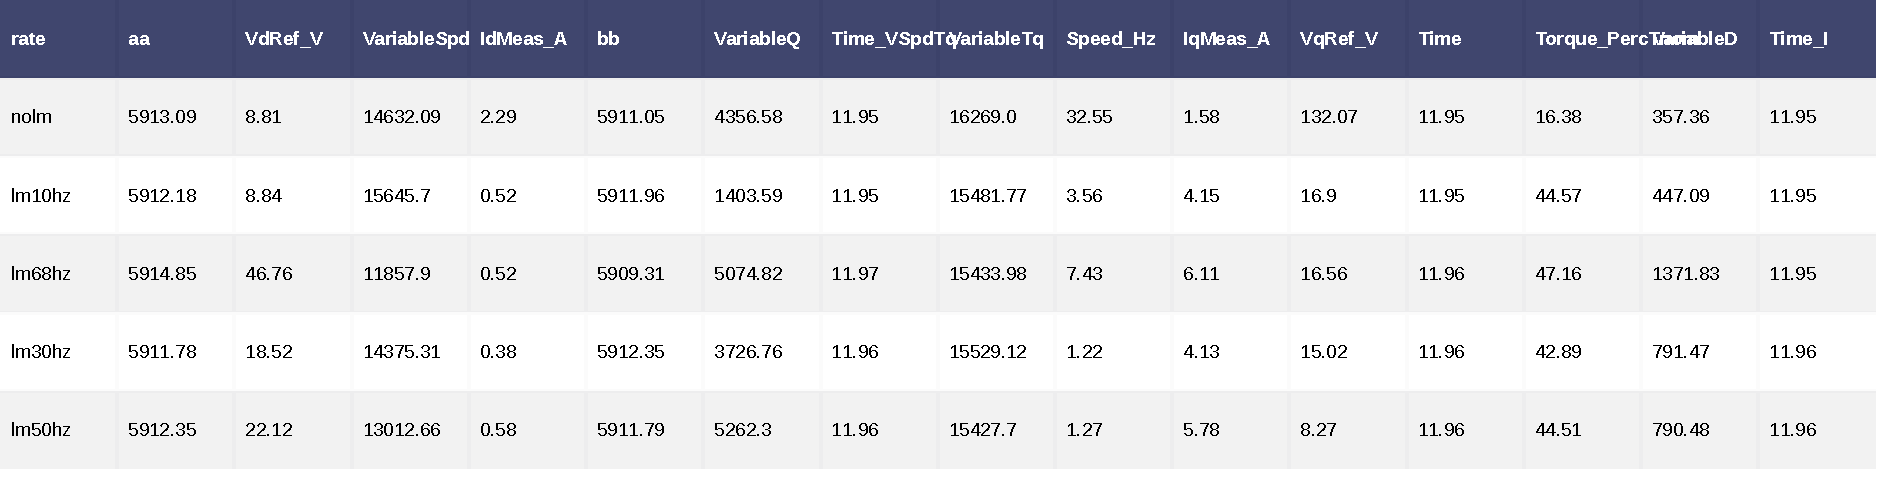
\includegraphics[width=1\linewidth]{std_values_of_features_in_dataset}}
        \caption{Standard Deviation Value of Features in the Dataset}
  \end{figure}

\section{Data Plots}

  \begin{figure}[H]
    \centering
      \href{https://plot.ly/~versag/14/#/}{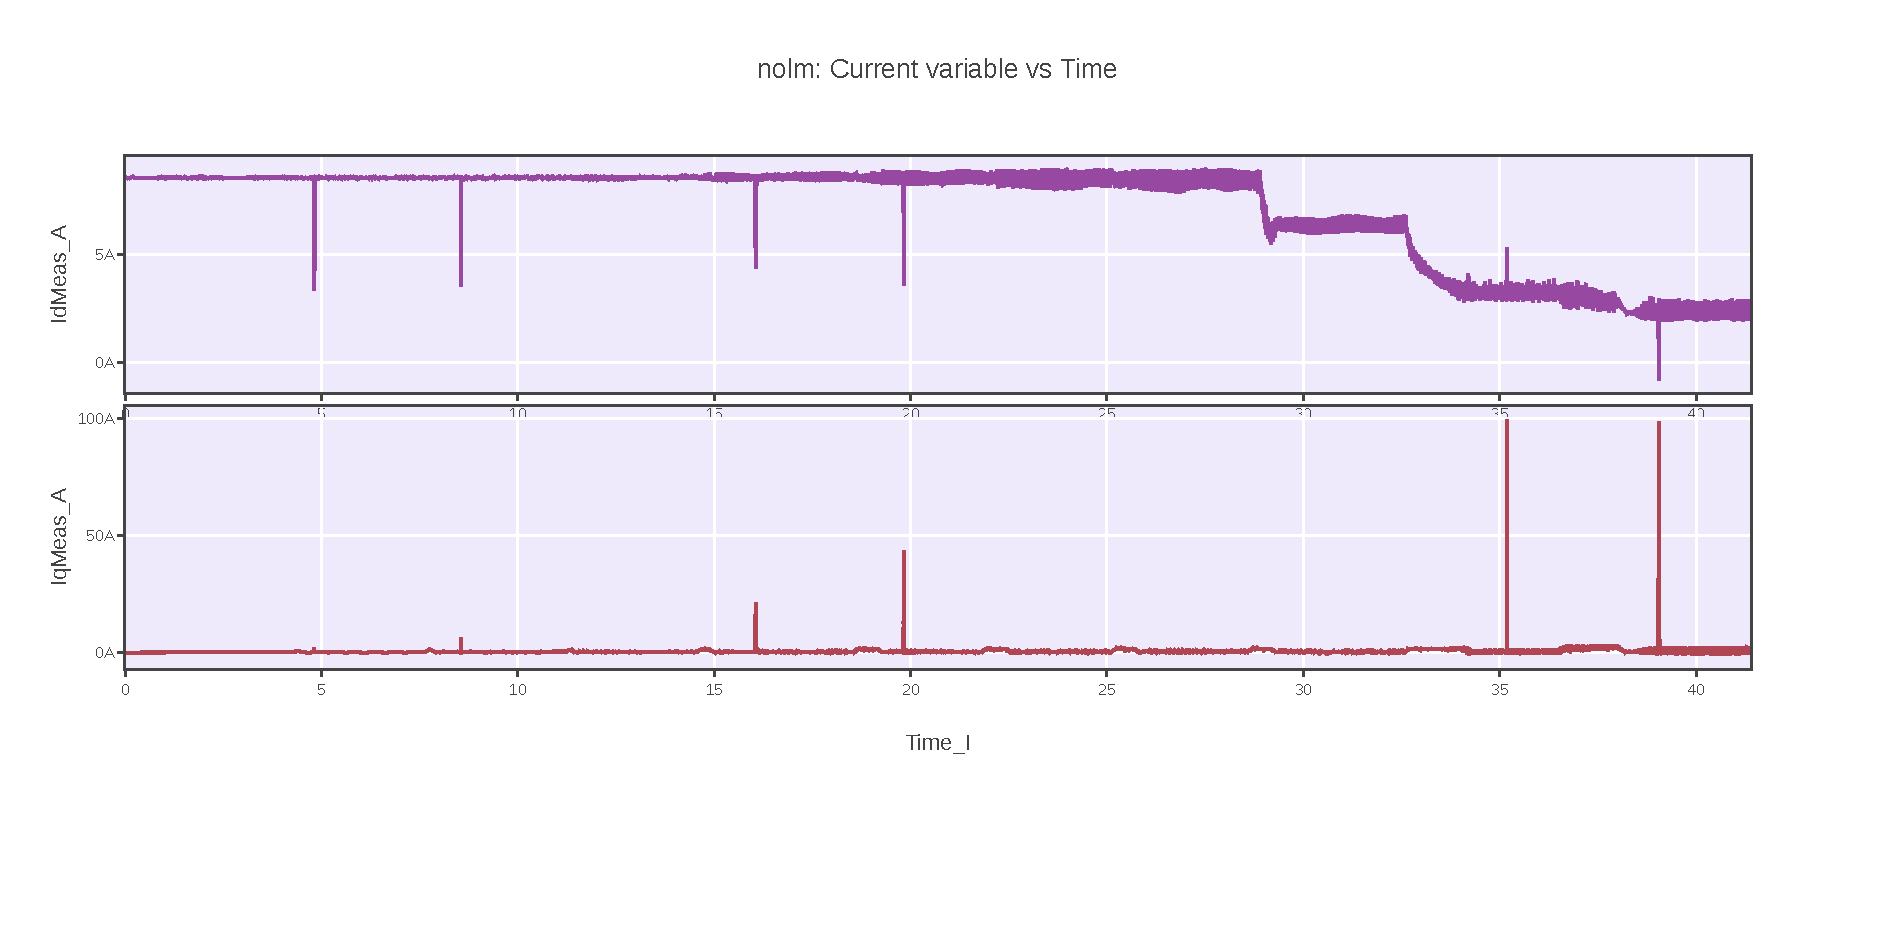
\includegraphics[width=1\linewidth]{nolm_current_vs_time}}
        \caption{nolm: current vs time}
  \end{figure}

  \begin{figure}[H]
    \centering
      \href{https://plot.ly/~versag/16/#/}{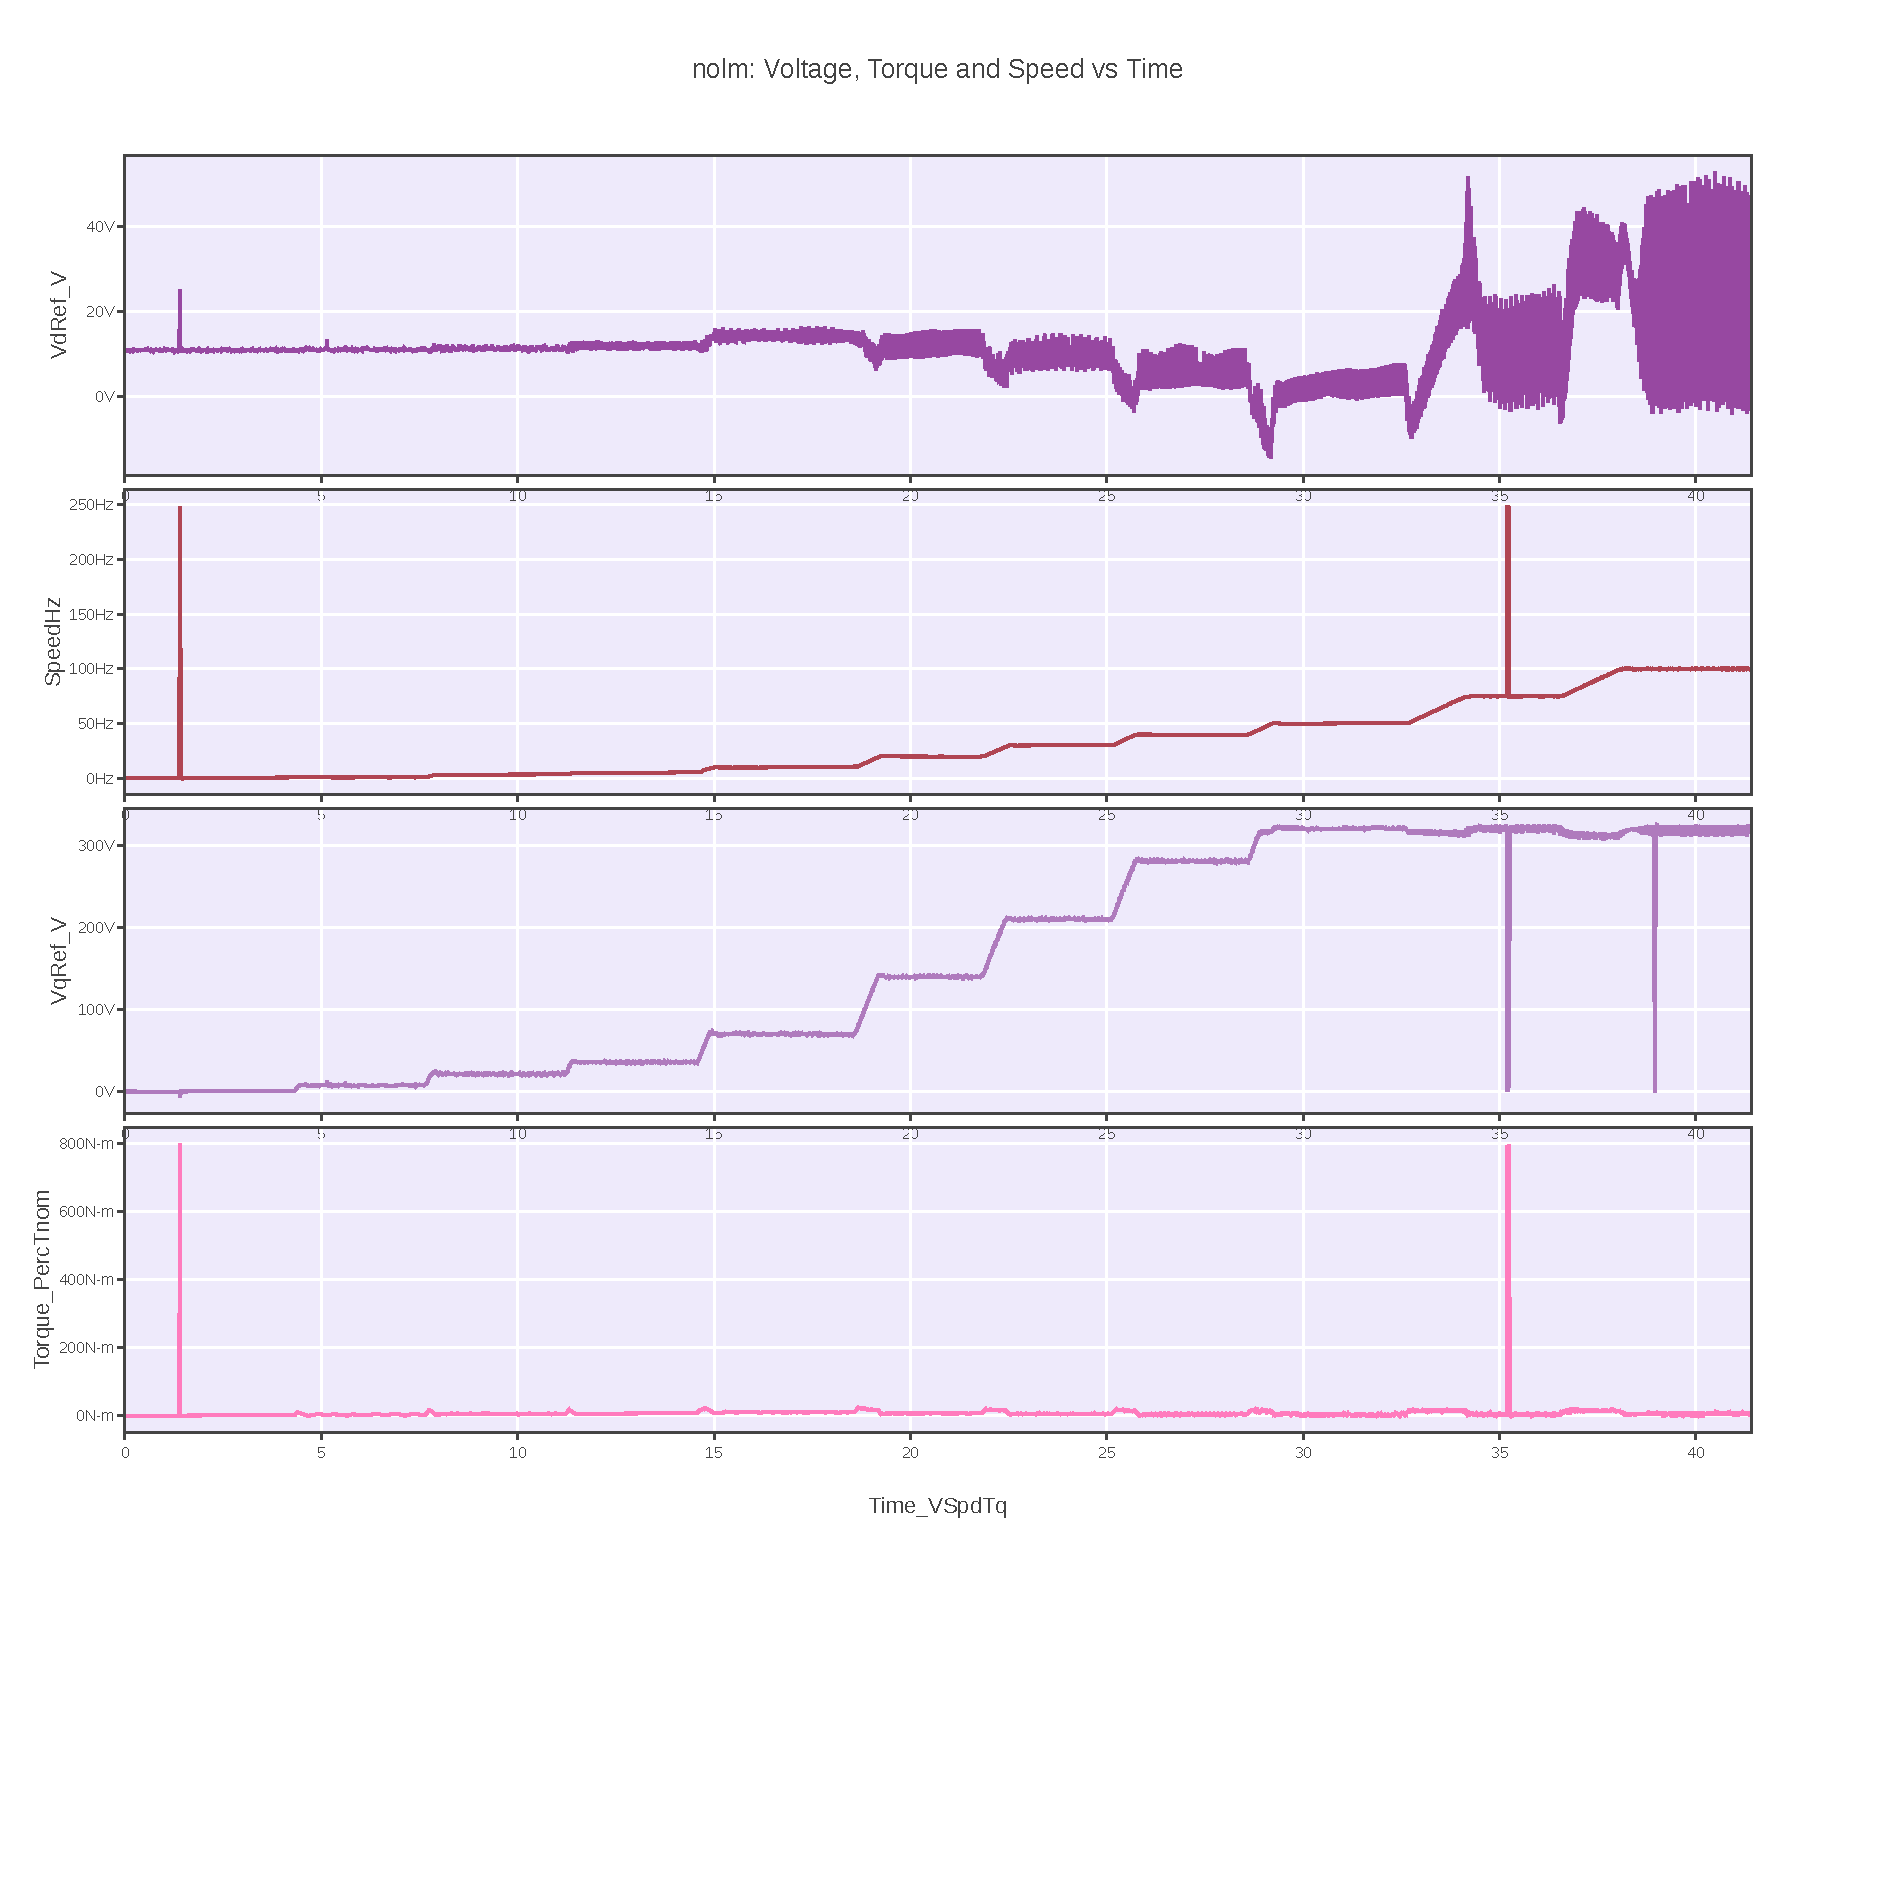
\includegraphics[width=1\linewidth]{nolm_voltage_torque_speed_vs_time}}
        \caption{nolm: voltage, torque and speed vs time}
  \end{figure}

  \begin{figure}[H]
    \centering
      \href{https://plot.ly/~versag/30/#/}{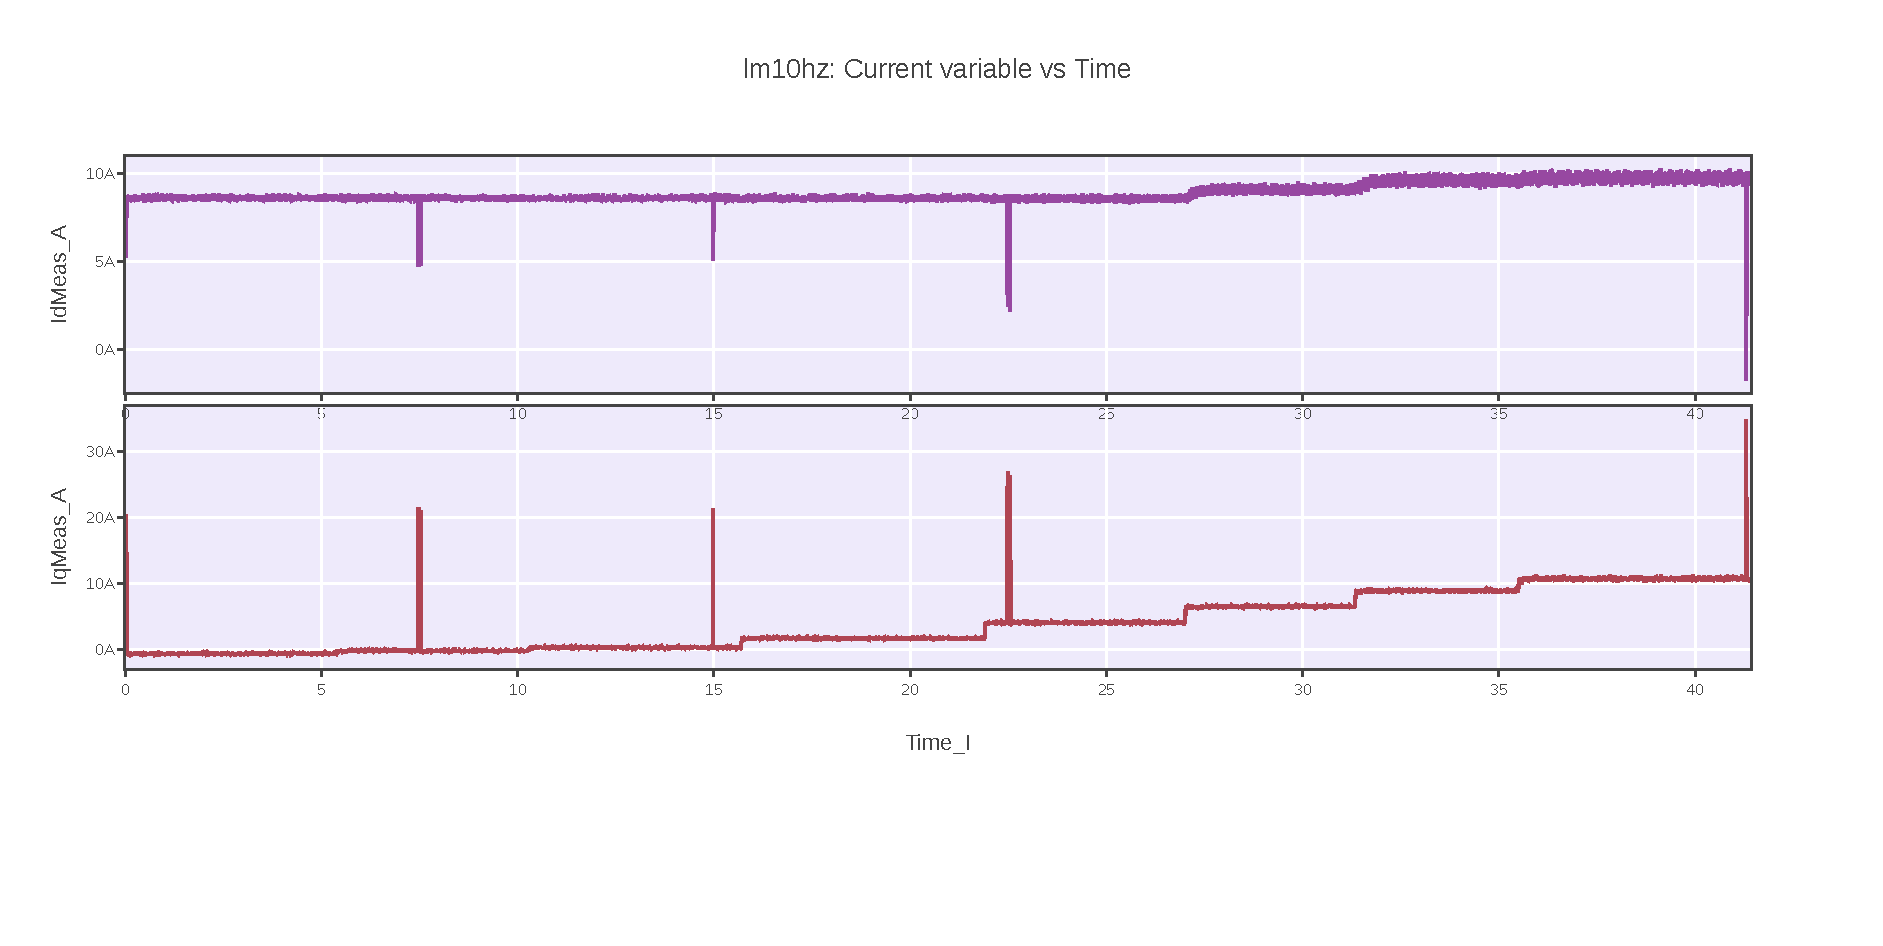
\includegraphics[width=1\linewidth]{lm10hz_current_vs_time}}
        \caption{lm10hz: current vs time}
  \end{figure}

  \begin{figure}[H]
    \centering
      \href{https://plot.ly/~versag/32/#/}{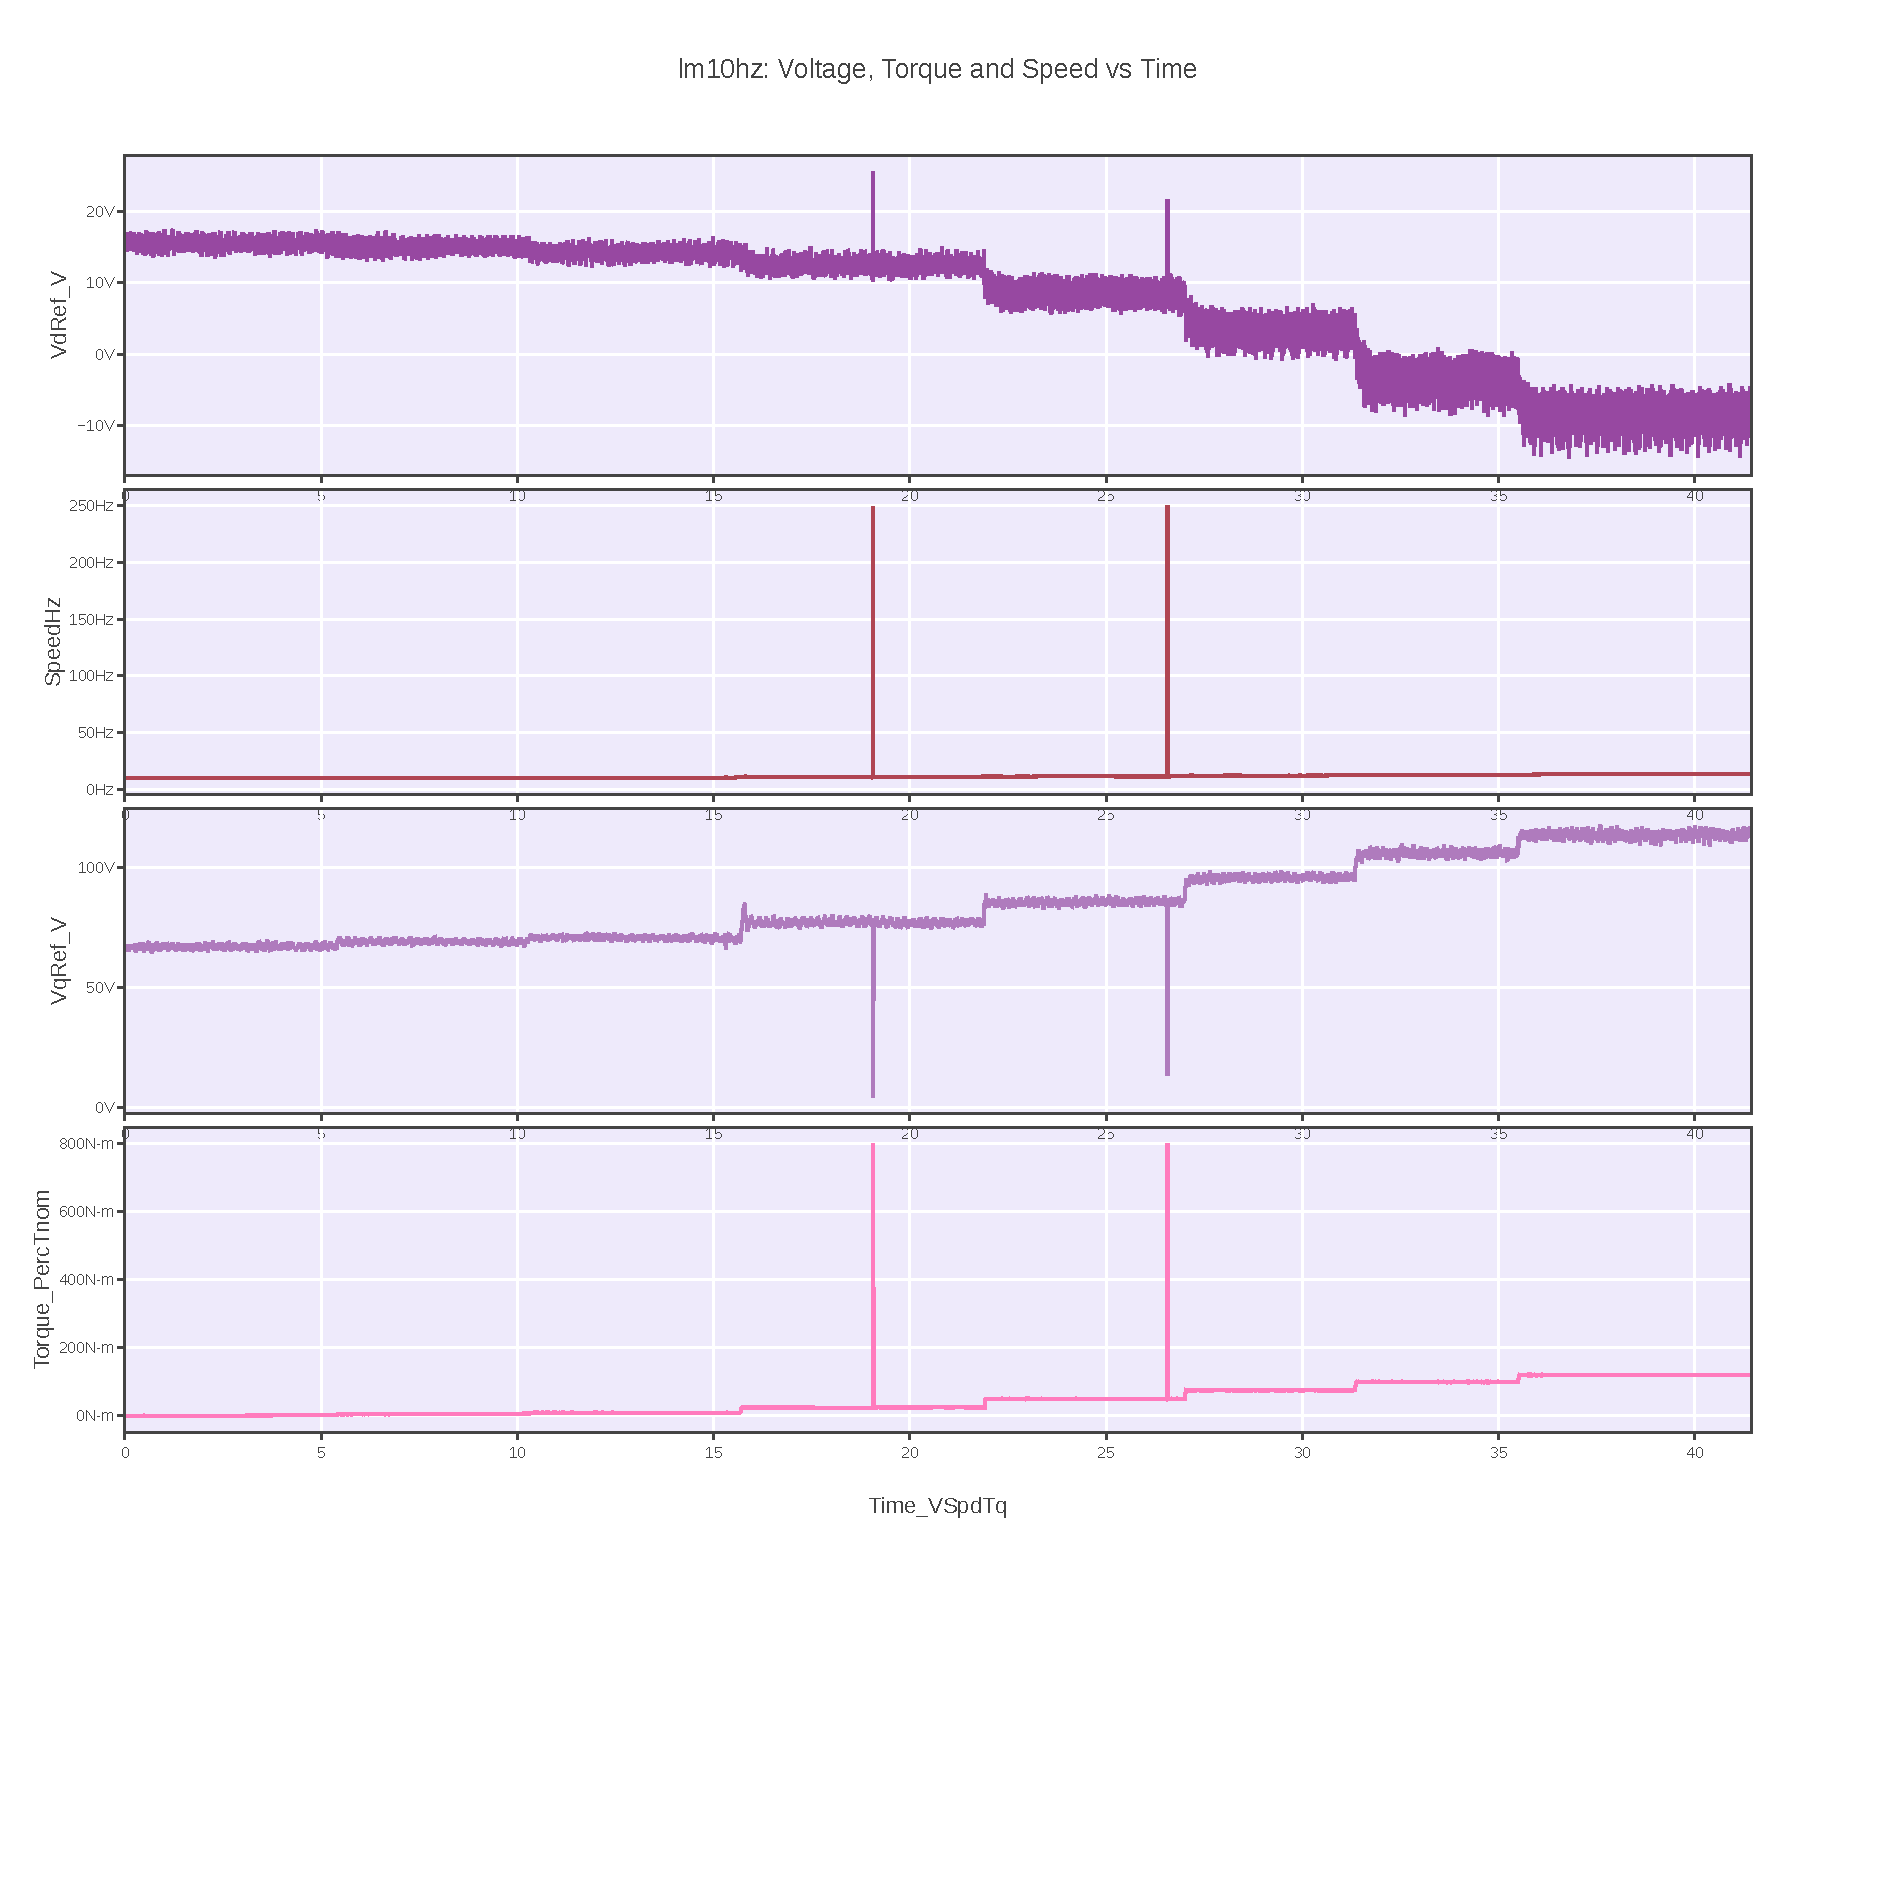
\includegraphics[width=1\linewidth]{lm10hz_voltage_torque_speed_vs_time}}
        \caption{lm10hz: voltage, torque and speed vs time}
  \end{figure}

  \begin{figure}[H]
    \centering
      \href{https://plot.ly/~versag/34/#/}{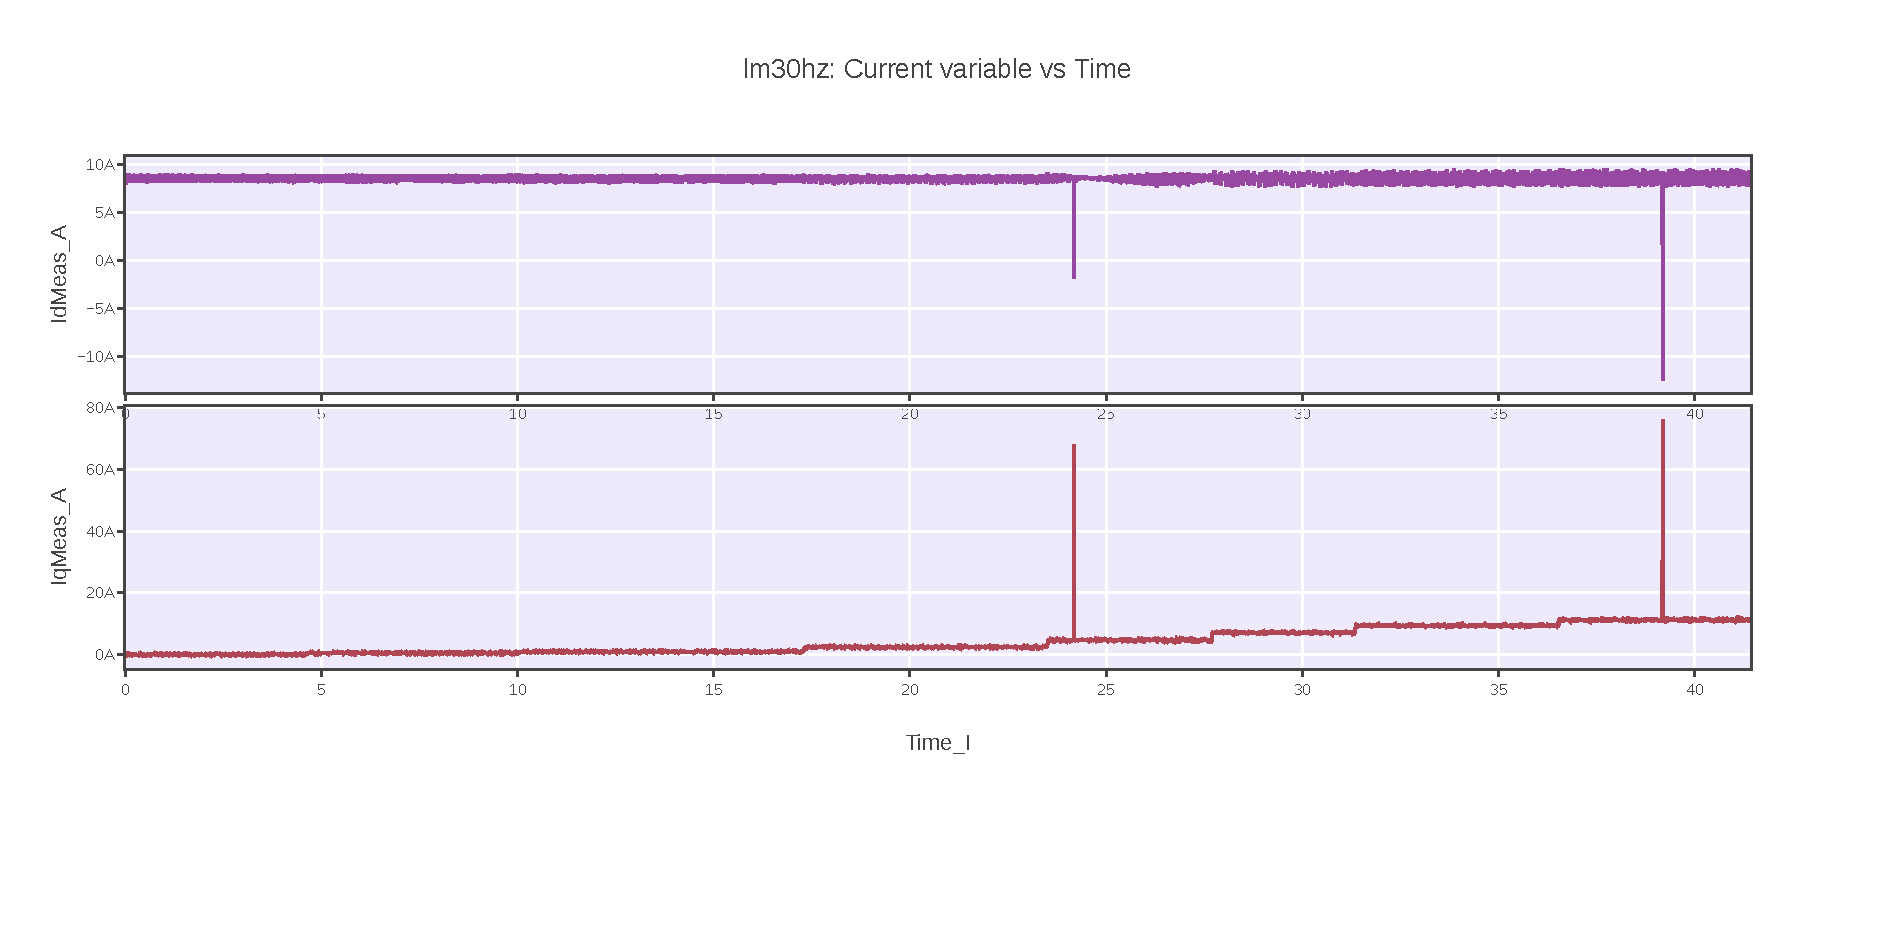
\includegraphics[width=1\linewidth]{lm30hz_current_vs_time}}
        \caption{lm30hz: current vs time}
  \end{figure}

  \begin{figure}[H]
    \centering
      \href{https://plot.ly/~versag/36/#/}{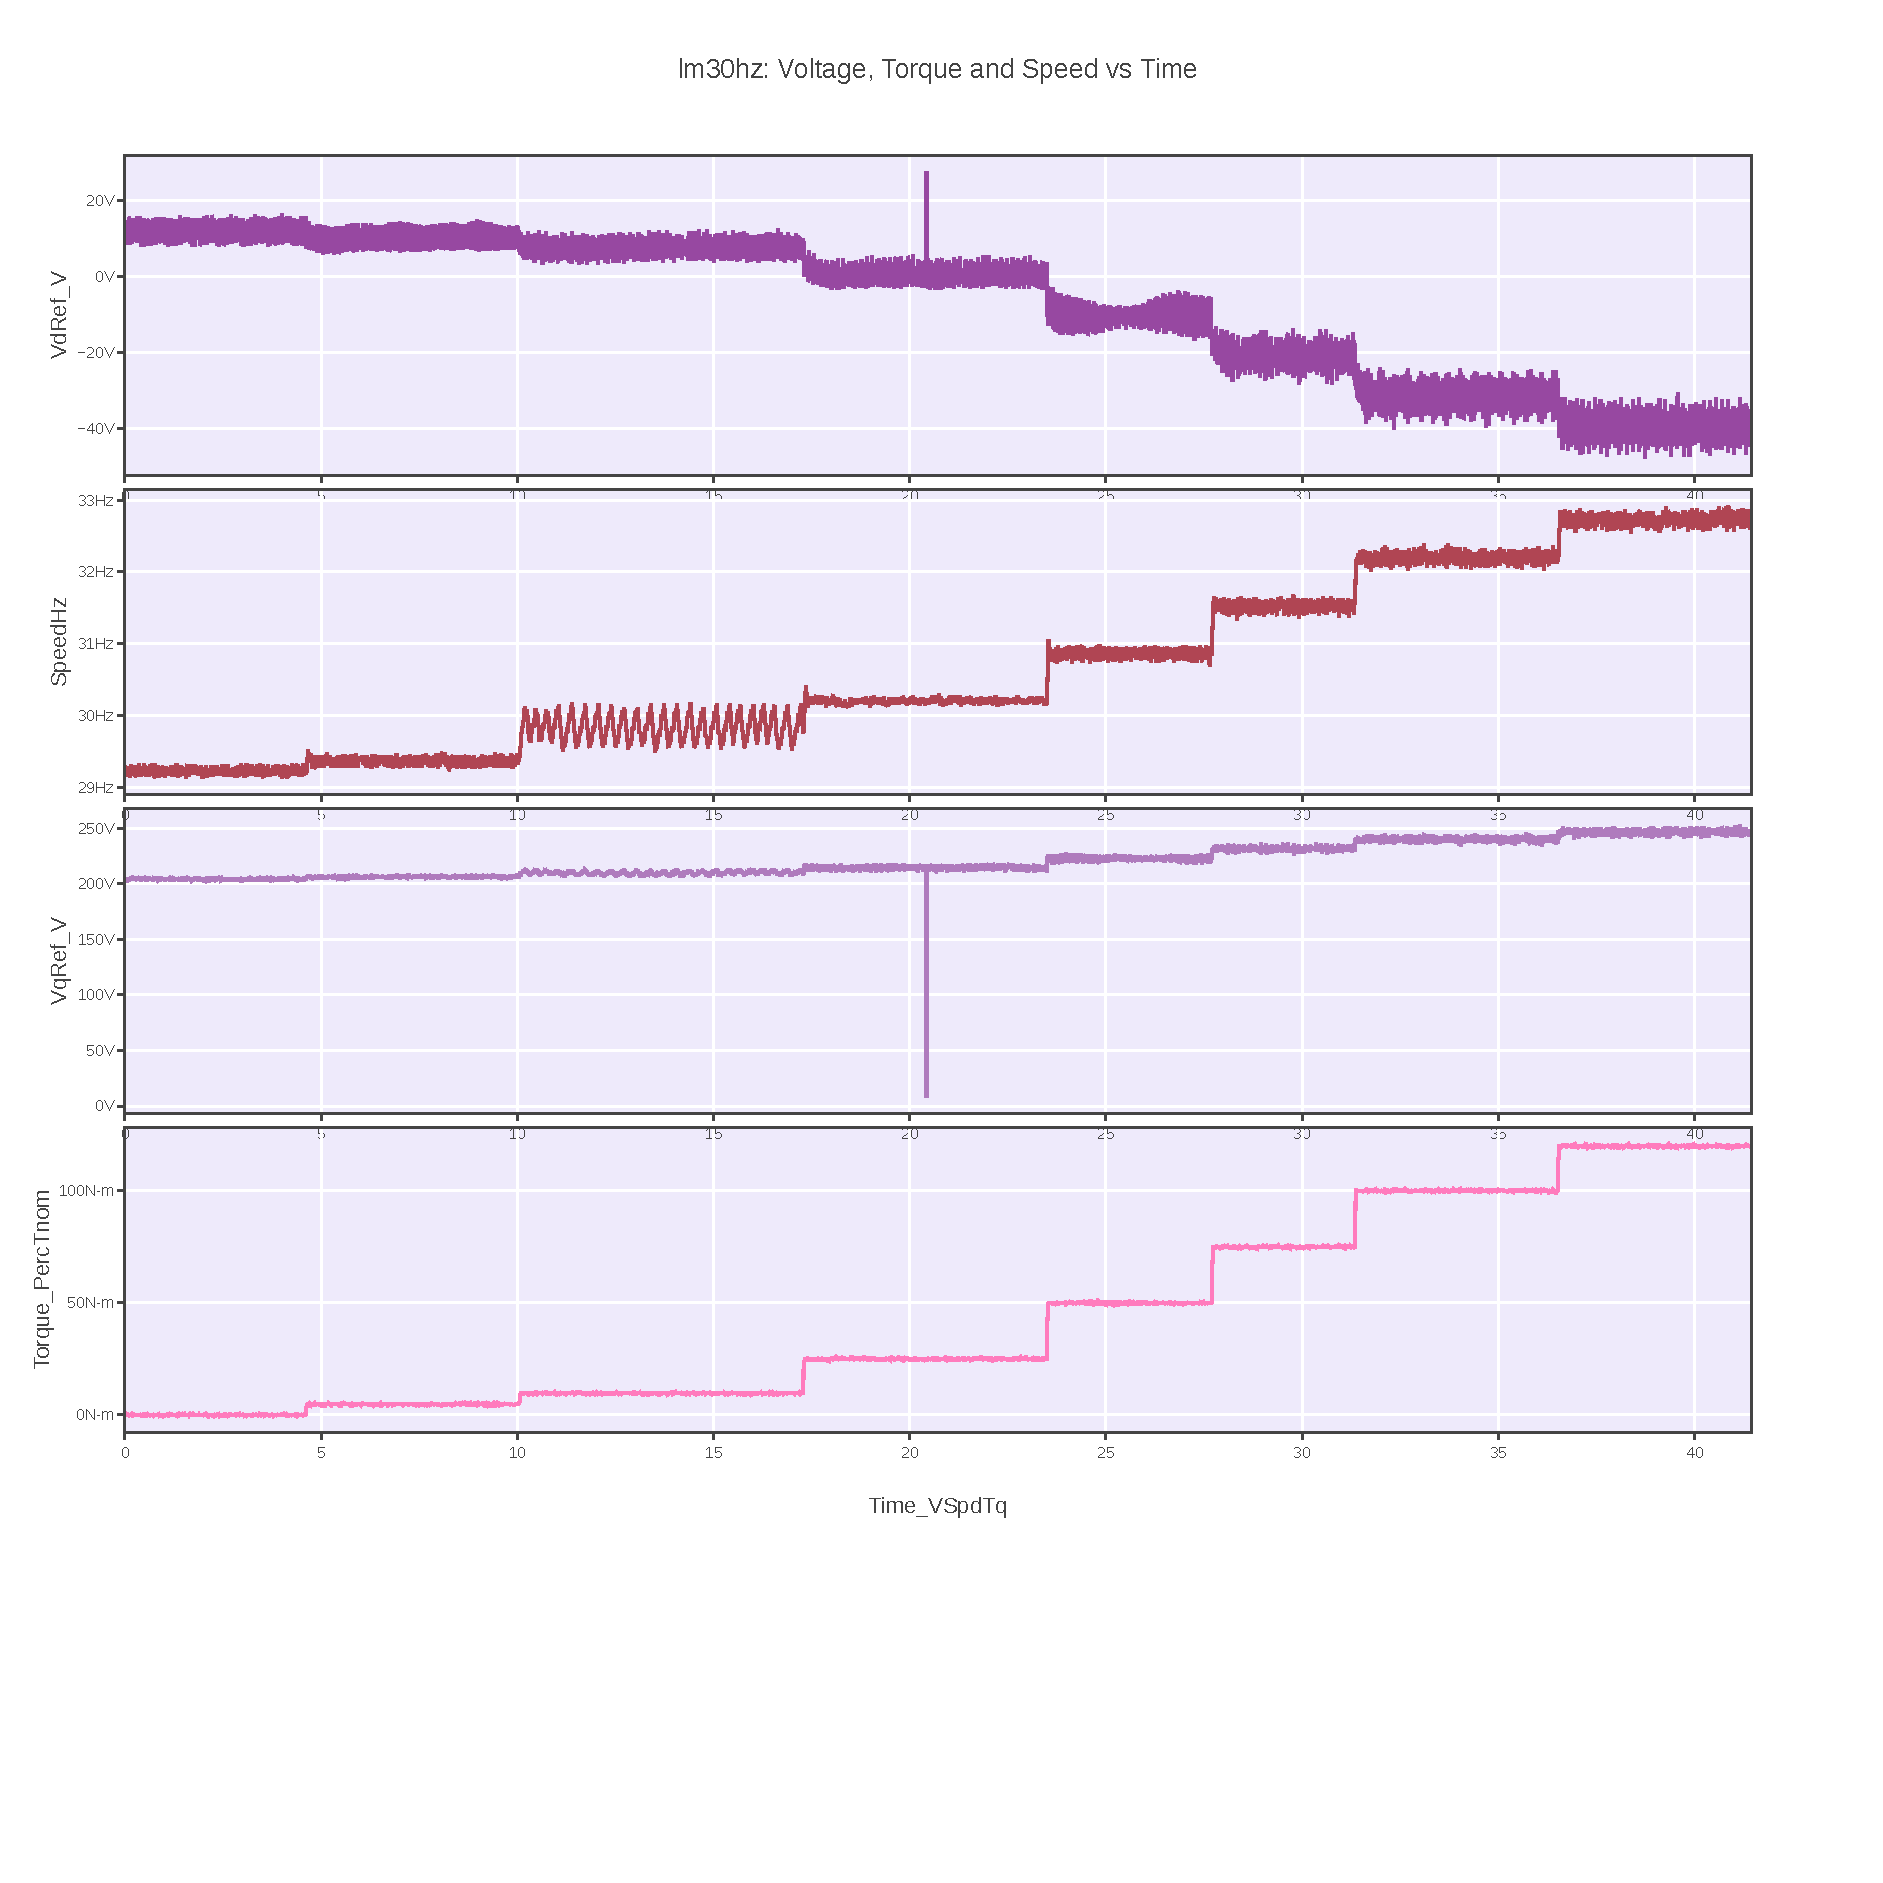
\includegraphics[width=1\linewidth]{lm30hz_voltage_torque_speed_vs_time}}
        \caption{lm30hz: voltage, torque and speed vs time}
  \end{figure}

  \begin{figure}[H]
    \centering
      \href{https://plot.ly/~versag/38/#/}{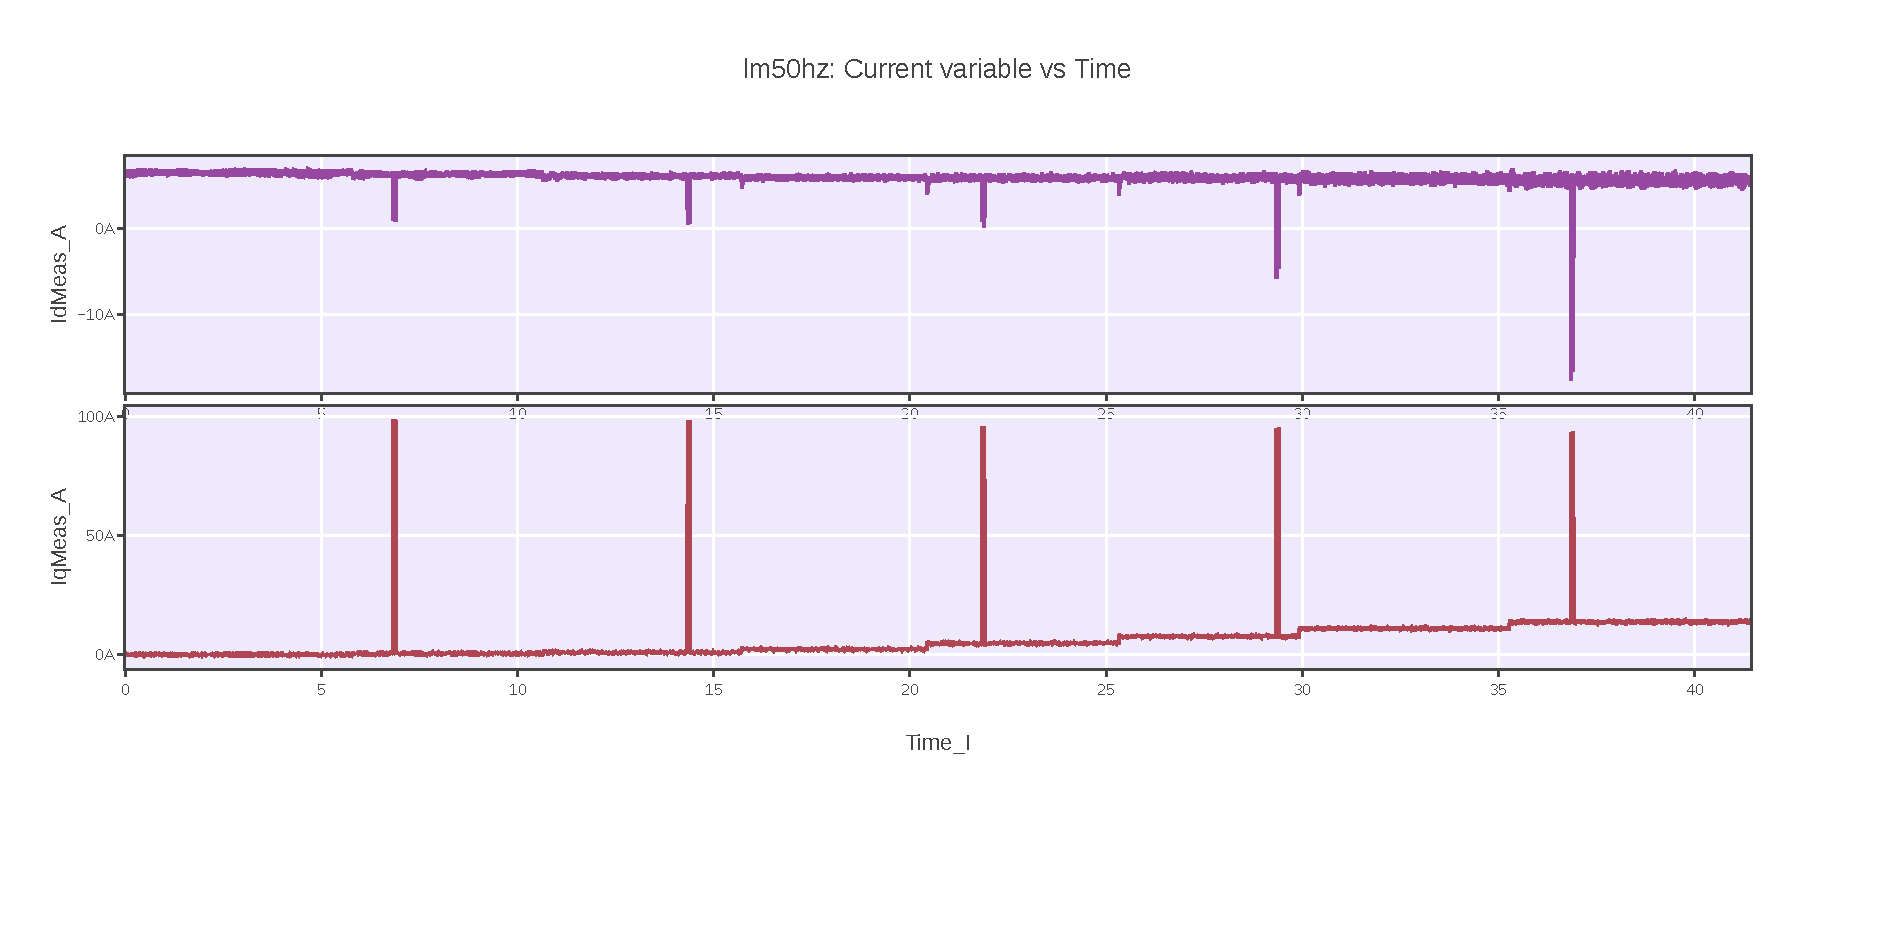
\includegraphics[width=1\linewidth]{lm50hz_current_vs_time}}
        \caption{lm50hz: current vs time}
  \end{figure}

  \begin{figure}[H]
    \centering
      \href{https://plot.ly/~versag/40/#/}{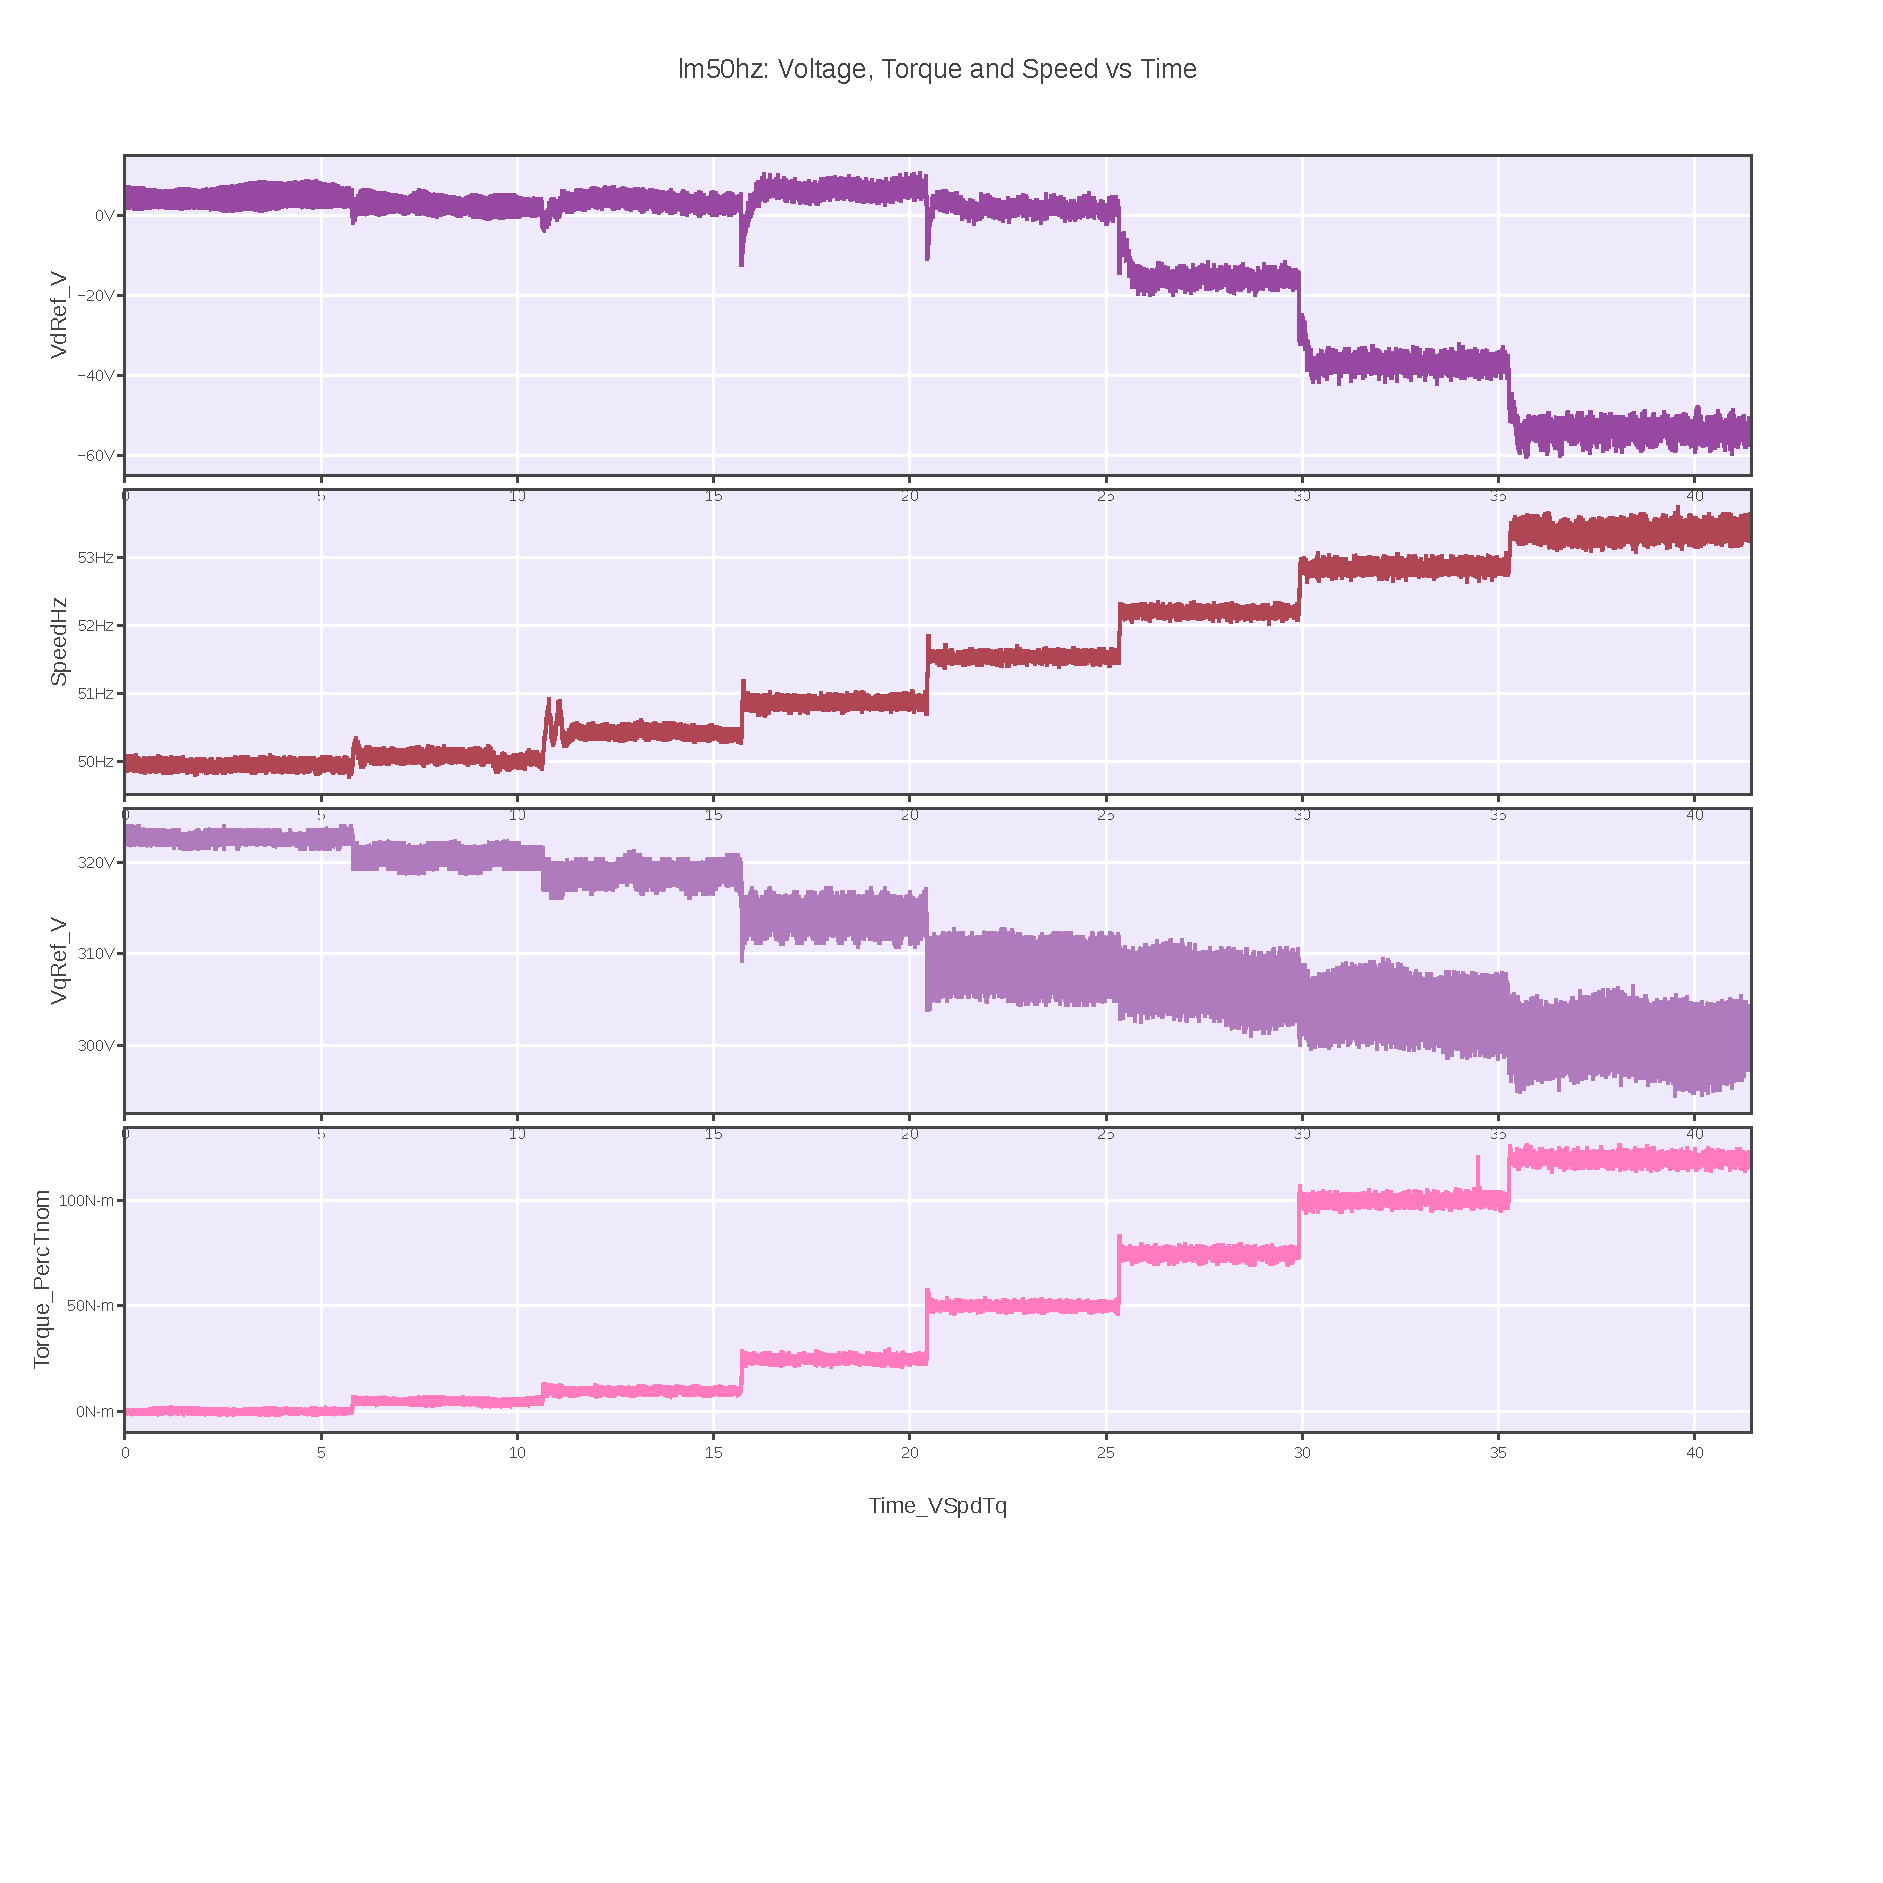
\includegraphics[width=1\linewidth]{lm50hz_voltage_torque_speed_vs_time}}
        \caption{lm50hz: voltage, torque and speed vs time}
  \end{figure}

  \begin{figure}[H]
    \centering
      \href{https://plot.ly/~versag/42/#/}{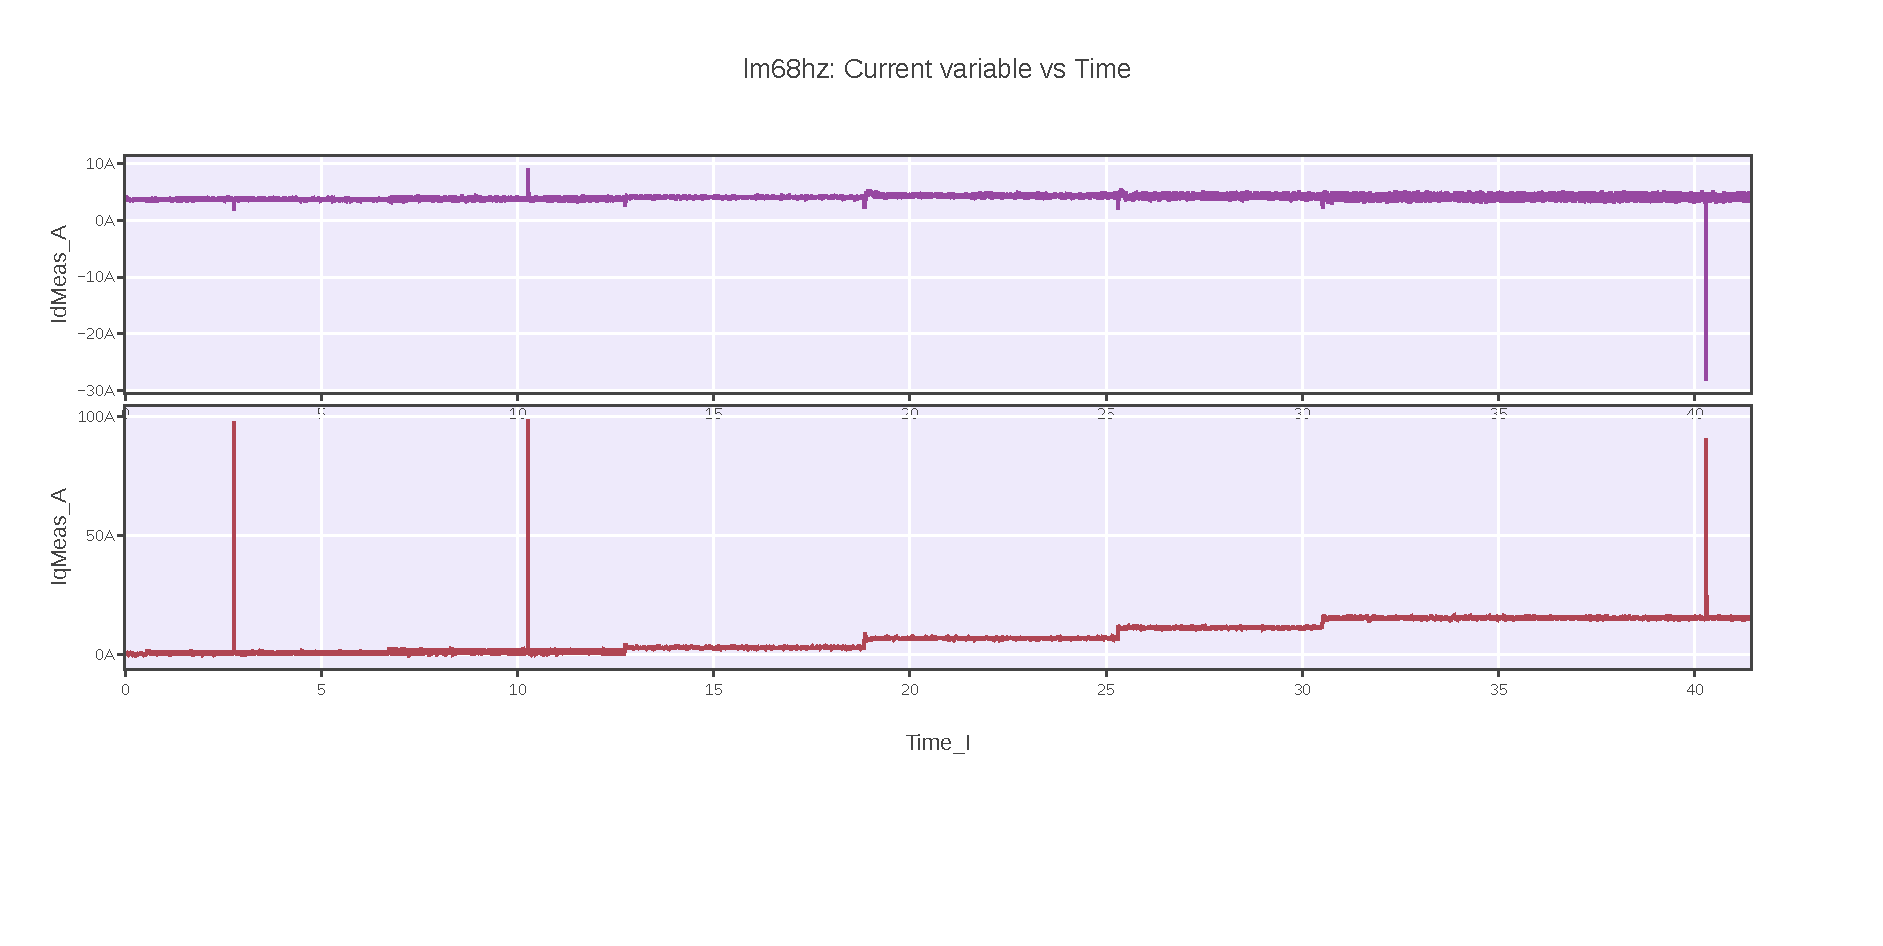
\includegraphics[width=1\linewidth]{lm68hz_current_vs_time}}
        \caption{lm68hz: current vs time}
  \end{figure}

  \begin{figure}[H]
    \centering
      \href{https://plot.ly/~versag/44/#/}{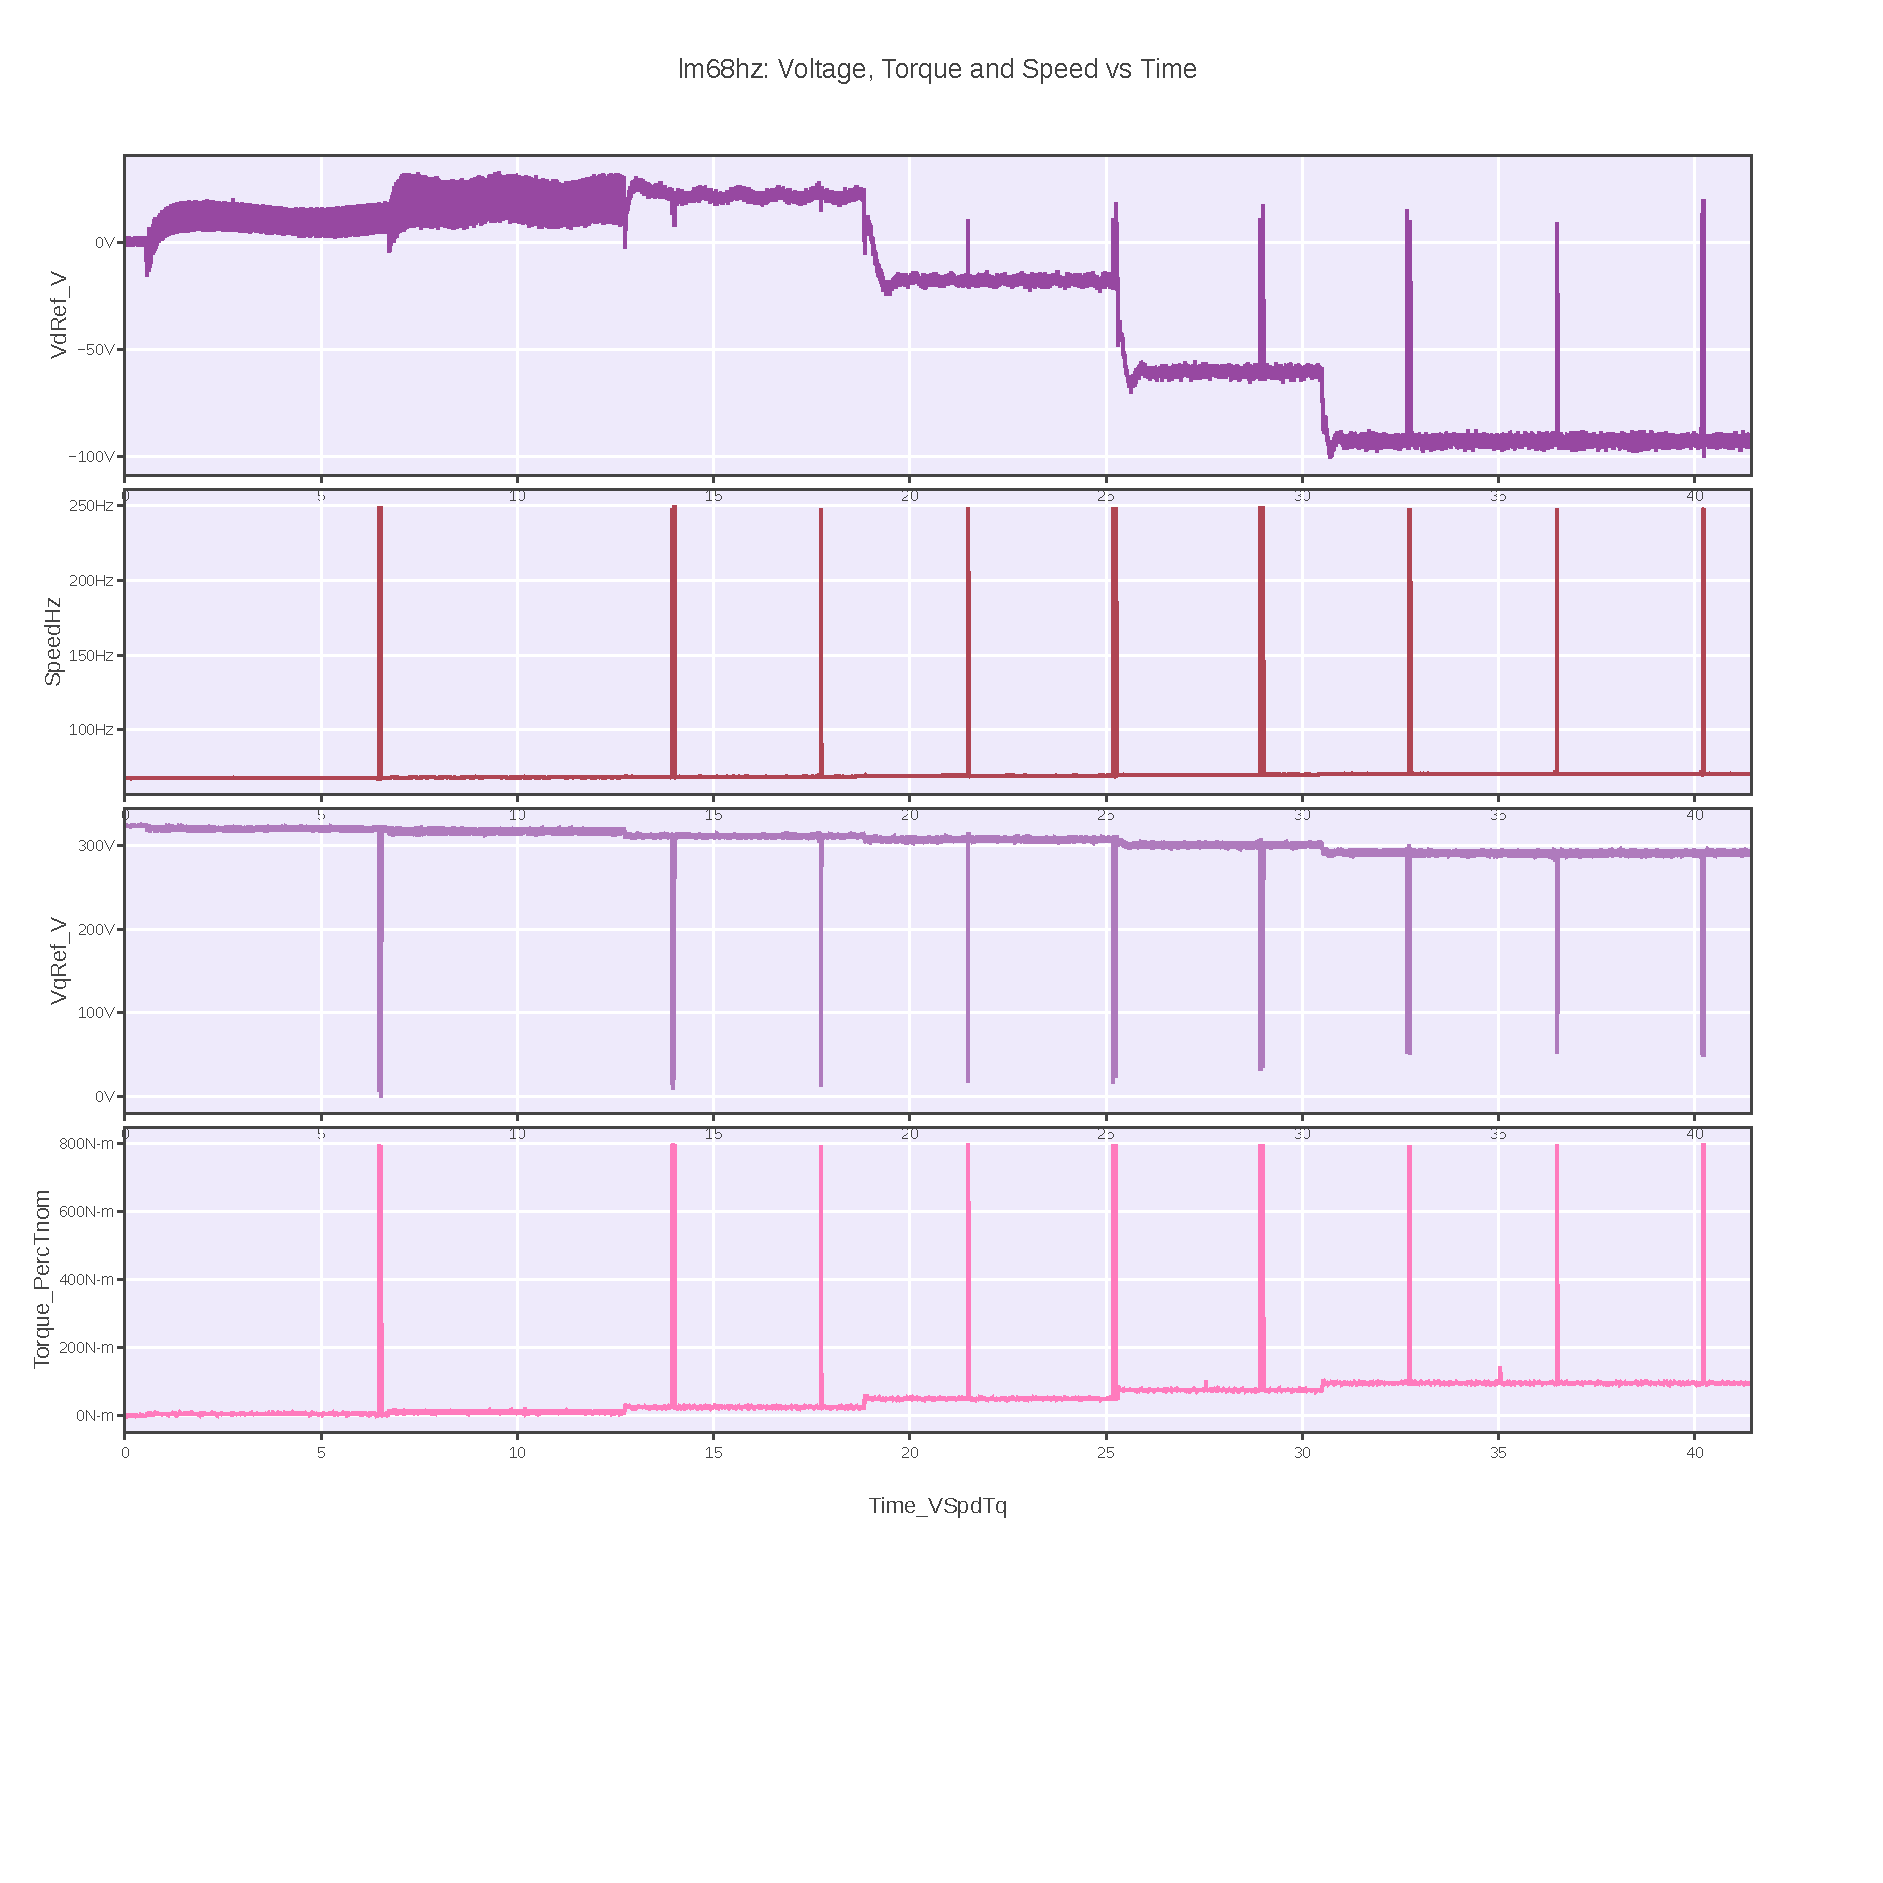
\includegraphics[width=1\linewidth]{lm68hz_voltage_torque_speed_vs_time}}
        \caption{lm68hz: voltage, torque and speed vs time}
  \end{figure}

\end{document}
